\subsection{Methodology}
\label{subsec:methodology}

To evaluate the Sobel filter implementations, we tested a grayscale image of size \(7112 \times 5146\). For the CPU OpenMP implementation, we experimented with thread counts of 1, 2, 4, 8, and 16 to observe the impact of varying concurrency levels on performance. For the CUDA GPU implementation, we evaluated our code with different configurations of threads per block \([32, 64, 128, 256, 512, 1024]\) and numbers of thread blocks \([1, 4, 16, 64, 256, 1024, 4096]\). For the OpenMP-offload code, we collected data from a single run.

We evaluated the performance of the Sobel filter implementations on both CPU and GPU platforms. To capture the necessary data for this analysis, we collected the following metrics: Runtime, Achieved Occupancy, and Percentage of Peak Sustained Memory Bandwidth.

Figure~\ref{fig:grayscale} shows the original grayscale image, while Figure~\ref{fig:sobel-output} displays the result after applying the Sobel filter.

\begin{figure}[h]
    \centering
    \begin{subfigure}{0.45\textwidth}
        \centering
        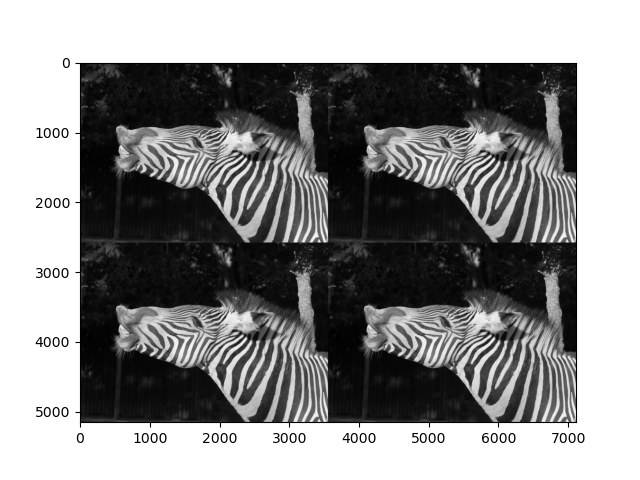
\includegraphics[width=\textwidth]{images/grayscale.png}
        \caption{Original Grayscale Image}
        \label{fig:grayscale}
    \end{subfigure}
    \hfill
    \begin{subfigure}{0.45\textwidth}
        \centering
        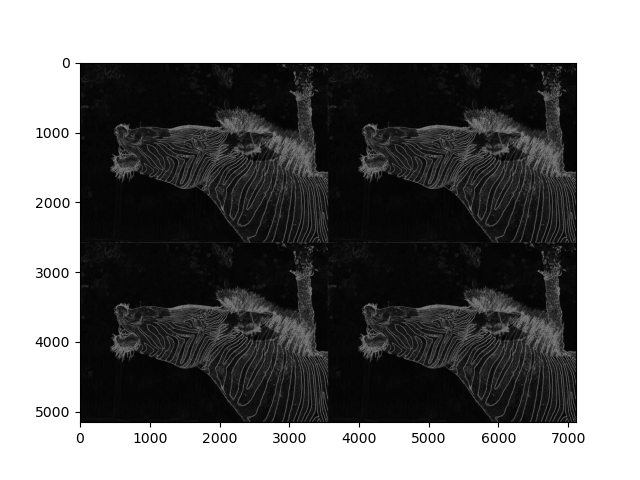
\includegraphics[width=\textwidth]{images/sobel_output.png}
        \caption{Sobel Filter Output}
        \label{fig:sobel-output}
    \end{subfigure}
    \caption{Example results showing the original grayscale image and the resulting image after applying the Sobel filter.}
    \label{fig:example-results}
\end{figure}

\subsubsection{Runtime}
\label{subsubsec:runtime}
\begin{itemize}
    \item \textbf{CPU:} The runtime on the CPU was measured using C++ \texttt{chrono\_timer()}, which surrounds the line of code calling the \texttt{do\_sobel\_filtering} function.
    \item \textbf{GPU:} For the GPU, runtime was recorded using the NVIDIA Compute Utility (\texttt{ncu}), which provides precise measurement of kernel execution time. This allows us to capture the duration of GPU processing without overhead from CPU-GPU data transfers.
\end{itemize}

\subsubsection{Achieved Occupancy}
\label{subsubsec:occupancy}
The achieved occupancy, a metric specific to GPU performance, was recorded using \texttt{ncu}. This value indicates the ratio of active warps to the maximum number of possible warps on a Streaming Multiprocessor during kernel execution, helping us understand how effectively the GPU resources were utilized.

\subsubsection{Percentage of Peak Sustained Memory Bandwidth}
\label{subsubsec:bandwidth}
This GPU-only metric, reported by \texttt{ncu}, measures the percentage of peak memory bandwidth utilized by the kernel. This value indicates how efficiently the Sobel filter accesses memory.
